\documentclass[]{article}
\usepackage{amsmath}
\usepackage{bm}
\usepackage{amssymb}
\usepackage{listings}
\usepackage{mathtools}
\usepackage{tikz}

\DeclarePairedDelimiter\floor{\lfloor}{\rfloor}

\lstset{columns=fullflexible,
	mathescape=true,
	numbers=left,
	stepnumber=1,
	literate=
	{=}{$\leftarrow{}$}{1},
	morekeywords={se,entao,para,devolva,continua},
	xleftmargin=5.0ex
}

\title{\vspace{-4.0cm}MAC0331 - Lista 1}
\author{Matheus T. de Laurentys, 9793714}

\begin{document}
	\maketitle
	\noindent
	\textbf{Q 1:} \\
	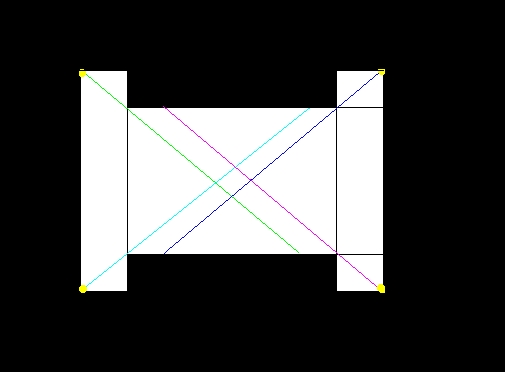
\includegraphics[scale=0.8]{lista2im.jpeg} \\
	\textbf{Q 12:} \\
	As seen in exercise 8, the dual of the triangulation of a polygon is a tree. Let $T$ be a triangulation of the polygon $P$ and $G$ be its associated (dual) tree. Let $G'$ be equal to $G$ after a rotation. There exists anther triangulation $T'$ of $P$ that is equal to $T$ except for a swap in the diagonal of a single quadrilateral formed by two adjacent triangles of $T$ such that $G'$ is its associated (dual) tree.
	
	In the context of triangulation/tree dual association, a rotation in $G$ is equivalent to a diagonal swap in $T$. \\
	\textbf{Q 13:}
	Professor Maqui Esperto is incorrect. The original proof goes as follow: choose any u,v,w consecutive vertices of P. Draw the line segment $\overline{uw}$. If it does not cross any edge of the polygon, it is a diagonal. If it does, move the segment towards $v$. If $t$ is the last vertex crossed, $\overline{vt}$ is a diagonal. The change does not work because there is no guarantee that $u$ and the new $t$ are not adjacent, let alone, that if they are not, that they form a diagonal.z
\end{document}